\chapter{Méthodes Non-Linéaires : Polynômes et Splines}
\section{Introduction et Motivation}

Le modèle de régression standard repose sur l'hypothèse d'une relation linéaire entre les variables prédictives $X$ et la variable cible $Y$ :
\begin{equation}
    Y = f(X) + \epsilon = \beta_0 + \beta_1 X_1 + \dots + \beta_p X_p + \epsilon 
\end{equation}
où $f$ est une fonction inconnue et $\epsilon$ est un terme d'erreur indépendant de $X$. 

Bien que les modèles linéaires soient simples à interpréter et à calculer, l'hypothèse de linéarité n'est souvent qu'une approximation. Pour améliorer la performance prédictive tout en conservant une certaine interprétabilité, nous pouvons explorer deux voies :
\begin{itemize}
    \item \textbf{Réduction de la complexité} : Méthodes de régularisation (Ridge, Lasso) pour réduire la variance.
    \item \textbf{Flexibilité non-linéaire} : Utilisation de polynômes, de fonctions en escalier ou de splines.
\end{itemize}

\section{Approche par Dictionnaires de Fonctions}

L'idée centrale pour modéliser une fonction non-linéaire $f$ est d'utiliser un développement sur un \textbf{dictionnaire} $\mathcal{D} = \{h_m\}_{m=1}^M$ :
\begin{equation}
    f(X) = \sum_{m=1}^{M} \beta_m h_m(X) 
\end{equation}

\subsection{Exemples de dictionnaires }
\begin{itemize}
    \item \textbf{Modèle Linéaire} : $h_m(x) = x_m$.
    \item \textbf{Modèle Polynomial} : $h_m(x) = x^m$.
    \item \textbf{Transformations log/racine} : $h_m(x) = \log(x_m)$ ou $\sqrt{x_m}$.
    \item \textbf{Séries de Fourier} : Base de sinus et cosinus pour les données périodiques.
    \item \textbf{Splines et Ondelettes} : Pour une flexibilité locale.
\end{itemize}

\begin{figure}[h]
    \centering
    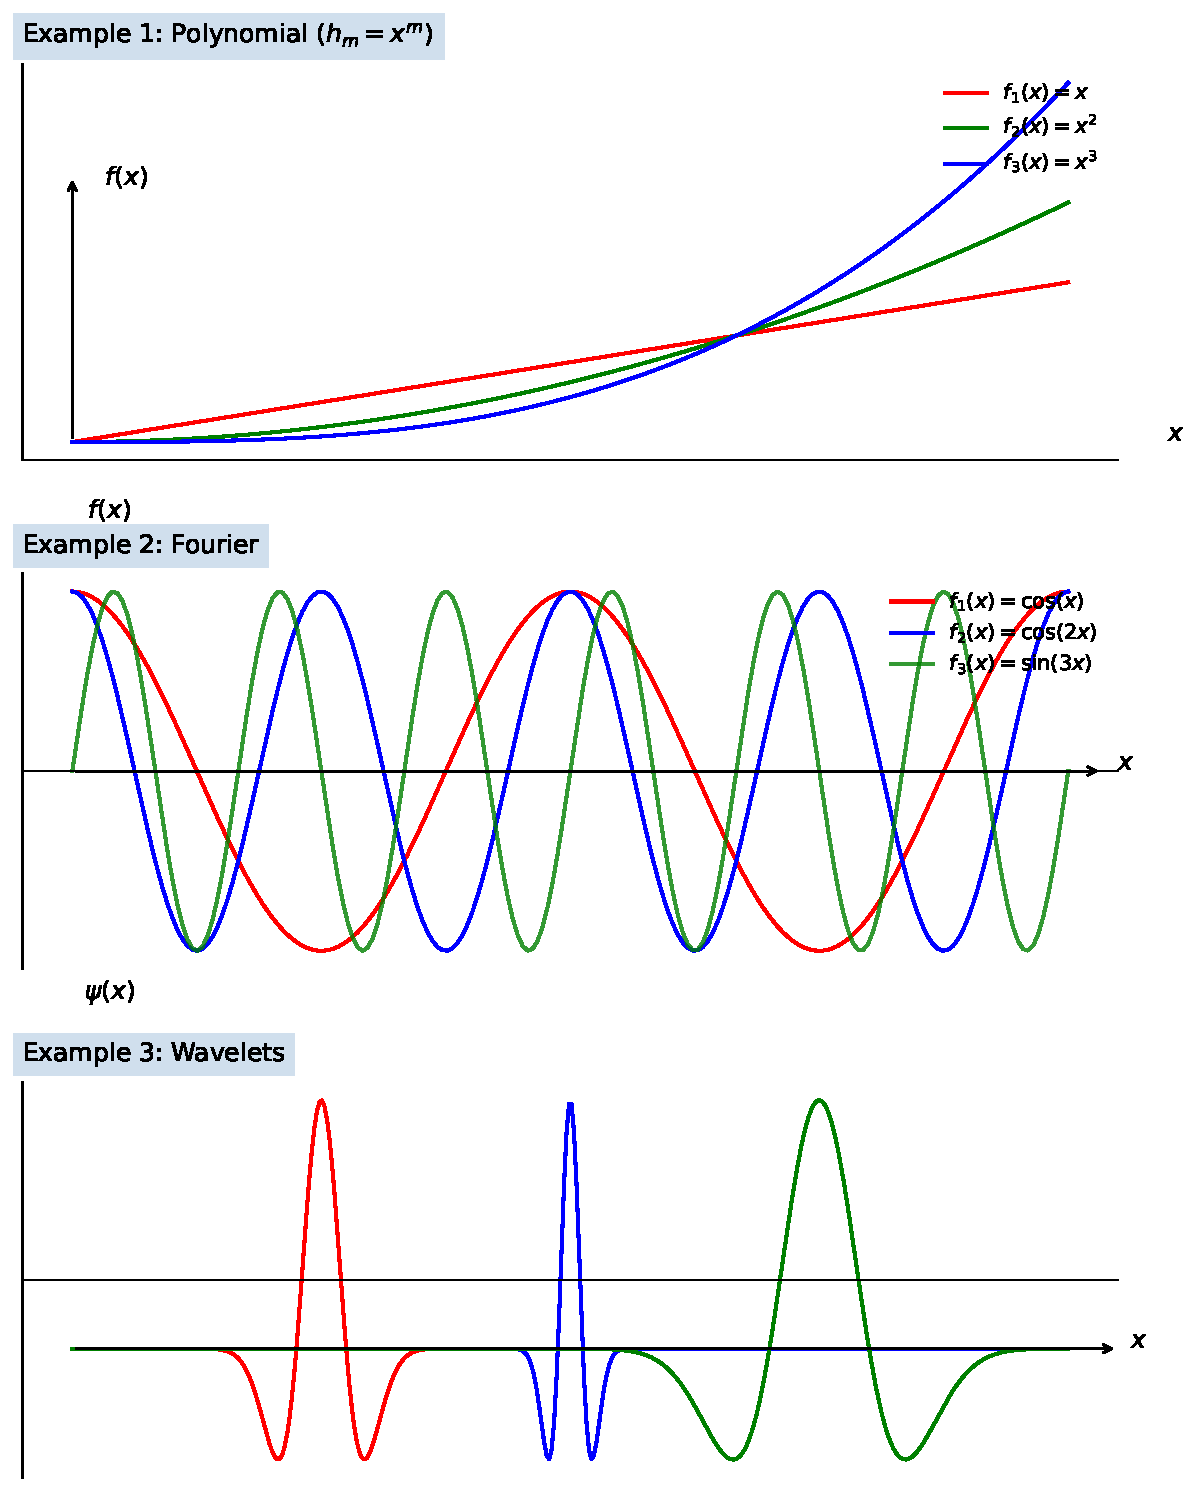
\includegraphics[width=\textwidth]{images/basis_functions.pdf}
    \caption{Exemples de fonctions de base (Polynômes, Splines, Ondelettes, Fourier, Fonctions en escalier).}
    \label{fig:basis_functions}
\end{figure}

\subsection{Construction du dictionnaire }
On peut construire ces ensembles par \textbf{restriction} (connaissance métier), par \textbf{sélection de modèle} (ne garder que les fonctions significatives) ou par \textbf{régularisation} (utiliser un grand dictionnaire avec des contraintes sur les coefficients).

\section{Régression Polynomiale}

\subsection{Définition et Forme Matricielle}
Le modèle polynomial d'ordre $m$ s'écrit:
\begin{equation}
    Y_i = \beta_0 + \beta_1 x_i + \beta_2 x_i^2 + \dots + \beta_m x_i^m + \epsilon_i
\end{equation}
Sous forme matricielle $Y = X_m \beta + \epsilon$, la matrice de design $X_m$ est une \textbf{matrice de Vandermonde}:
\begin{equation}
    X_m = \begin{pmatrix} 1 & x_1 & \dots & x_1^m \\ \vdots & \vdots & \ddots & \vdots \\ 1 & x_n & \dots & x_n^m \end{pmatrix}
\end{equation}
L'estimateur des moindres carrés est $\hat{\beta} = (X_m^T X_m)^{-1} X_m^T Y$.

\subsection{Orthonormalisation (Gram-Schmidt)}
L'utilisation directe des puissances $x^k$ peut entraîner une forte colinéarité. On préfère souvent utiliser des \textbf{polynômes orthogonaux} $h_k(x)$ tels que $\langle h_k, h_l \rangle = \delta_{kl}$. En R, la fonction \texttt{poly(x, degree)} effectue cette transformation par défaut.

\subsection{Risque et Compromis Biais-Variance}
L'erreur quadratique moyenne (MSE) se décompose en:
\begin{equation}
    MSE(\hat{f}) = \text{Biais}^2(\hat{f}) + \text{Var}(\hat{f})
\end{equation}
Augmenter le degré du polynôme réduit le biais mais augmente la variance. Un degré trop élevé conduit au \textbf{sur-apprentissage} (overfitting) ou "polynomial wiggle".

\begin{figure}[h]
    \centering
    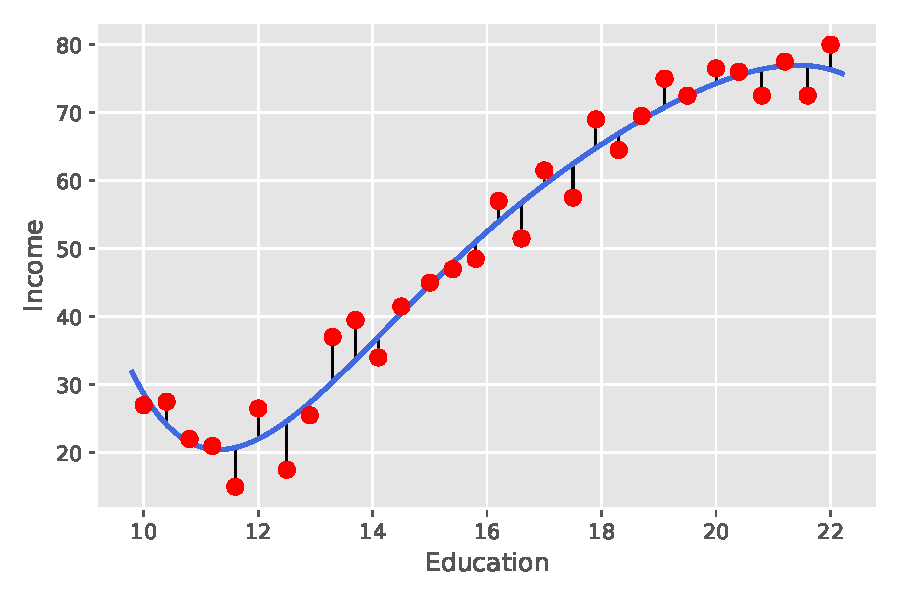
\includegraphics[width=0.6\textwidth]{images/income_poly.pdf}
    \caption{Exemple de modèle polynomial de degré 5. Un degré trop élevé peut conduire à des oscillations importantes aux bornes ("polynomial wiggle").}
    \label{fig:income_poly}
\end{figure}

\begin{figure}[h]
    \centering
    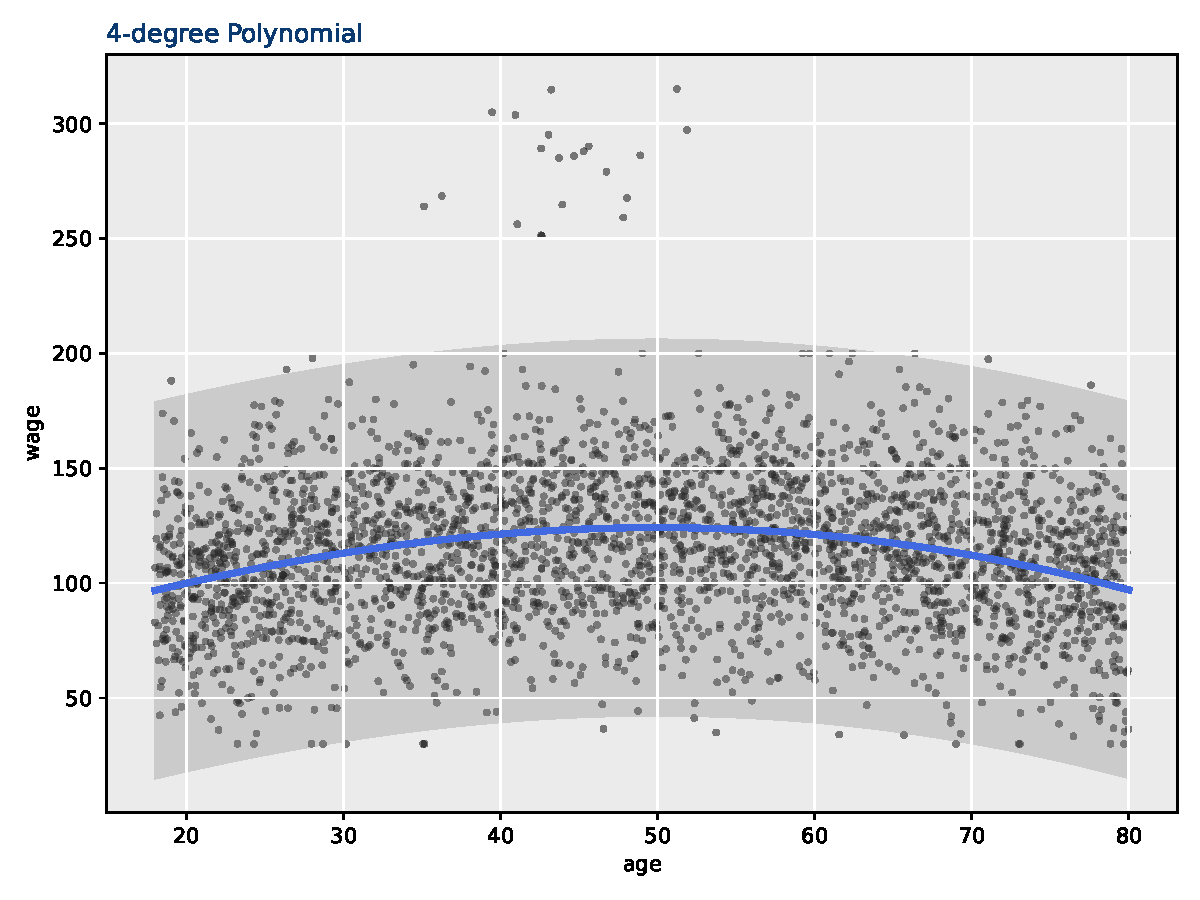
\includegraphics[width=0.8\textwidth]{images/wage_poly.pdf}
    \caption{Régression polynomiale et fonctions en escalier sur le jeu de données Wage.}
    \label{fig:wage_poly}
\end{figure}

\begin{figure}[h]
    \centering
    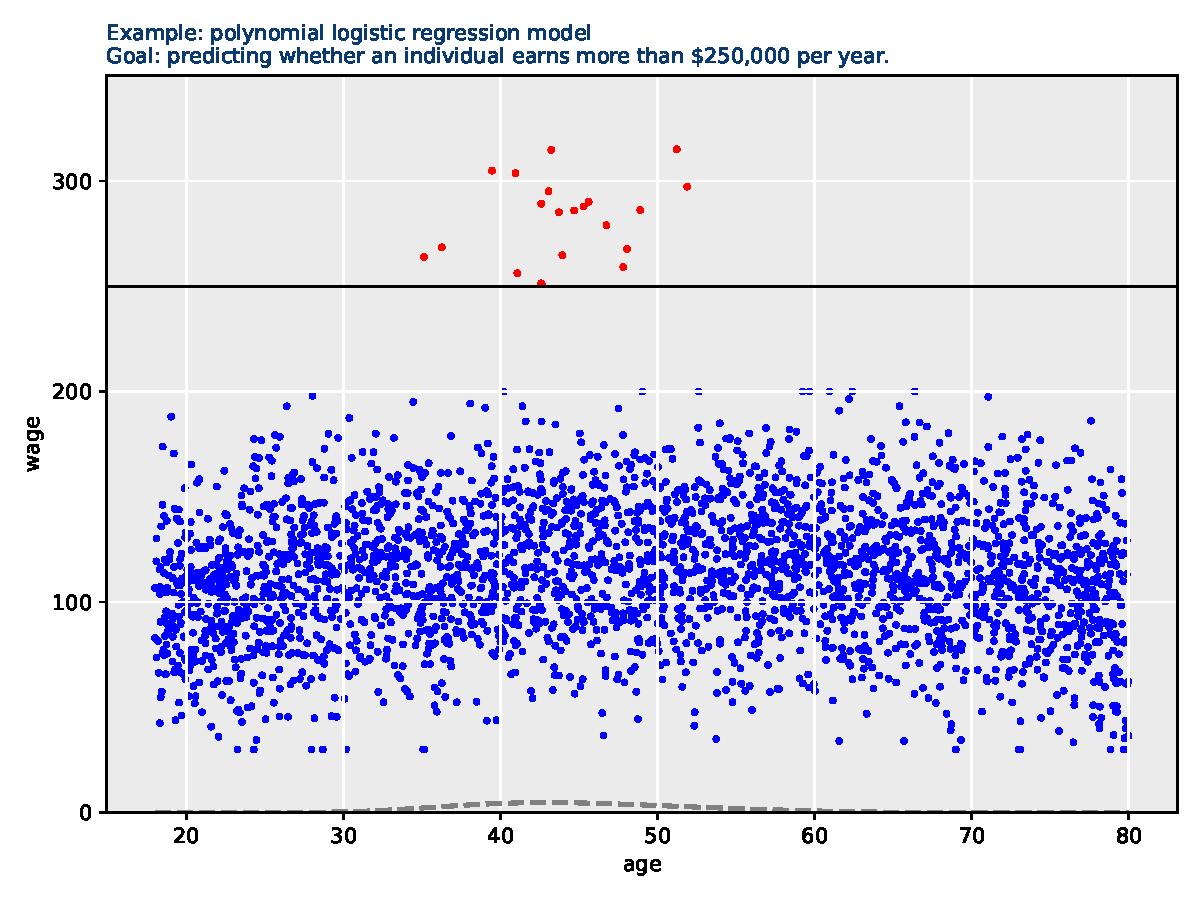
\includegraphics[width=0.8\textwidth]{images/wage_logistic.pdf}
    \caption{Régression logistique polynomiale sur le jeu de données Wage.}
    \label{fig:wage_logistic}
\end{figure}

\section{Sélection de Modèle}

Le risque empirique (RSS) diminue toujours avec la complexité. Pour choisir le degré optimal $m$, on utilise des critères pénalisés ou la validation croisée:
\begin{itemize}
    \item \textbf{Statistique $C_p$ de Mallows / AIC} : $R_n(\hat{f}_m) + 2\frac{\sigma^2(m+1)}{n}$.
    \item \textbf{ANOVA} : Pour tester si un modèle $\mathcal{M}_{m+1}$ apporte une amélioration significative par rapport à $\mathcal{M}_m$ (modèles emboîtés).
\end{itemize}

\section{Splines de Régression}

\subsection{Fonctions constantes par morceaux}
Au lieu d'imposer une structure globale, on divise le support de $X$ en segments via des \textbf{nœuds} (knots) $\xi_1, \dots, \xi_K$. 
Dans chaque intervalle, on ajuste une constante. Le dictionnaire est alors composé de fonctions indicatrices $h_m(x) = I(\xi_m \le x < \xi_{m+1})$.

\subsection{Splines Polynomiales et Continuité}
\begin{itemize}
    \item \textbf{Polynômes par morceaux} : On ajuste un polynôme (ex: cubique) dans chaque segment. Sans contraintes, la fonction est discontinue aux nœuds.
    \item \textbf{Splines de degré $d$} : Ce sont des polynômes par morceaux de degré $d$ possédant des dérivées continues aux nœuds. La régression spline est donc une régression polynomiale par morceaux \textbf{($\bigstar$ EXAMEN) avec des contraintes (de continuité) aux nœuds} (\textit{with constraints at nodes}).
    \item \textbf{Splines Cubiques ($d=3$)} : Les plus utilisées. Elles assurent la continuité de la fonction, de la pente (1ère dérivée) et de la courbure (2ème dérivée).
\end{itemize}

\begin{figure}[h]
    \centering
    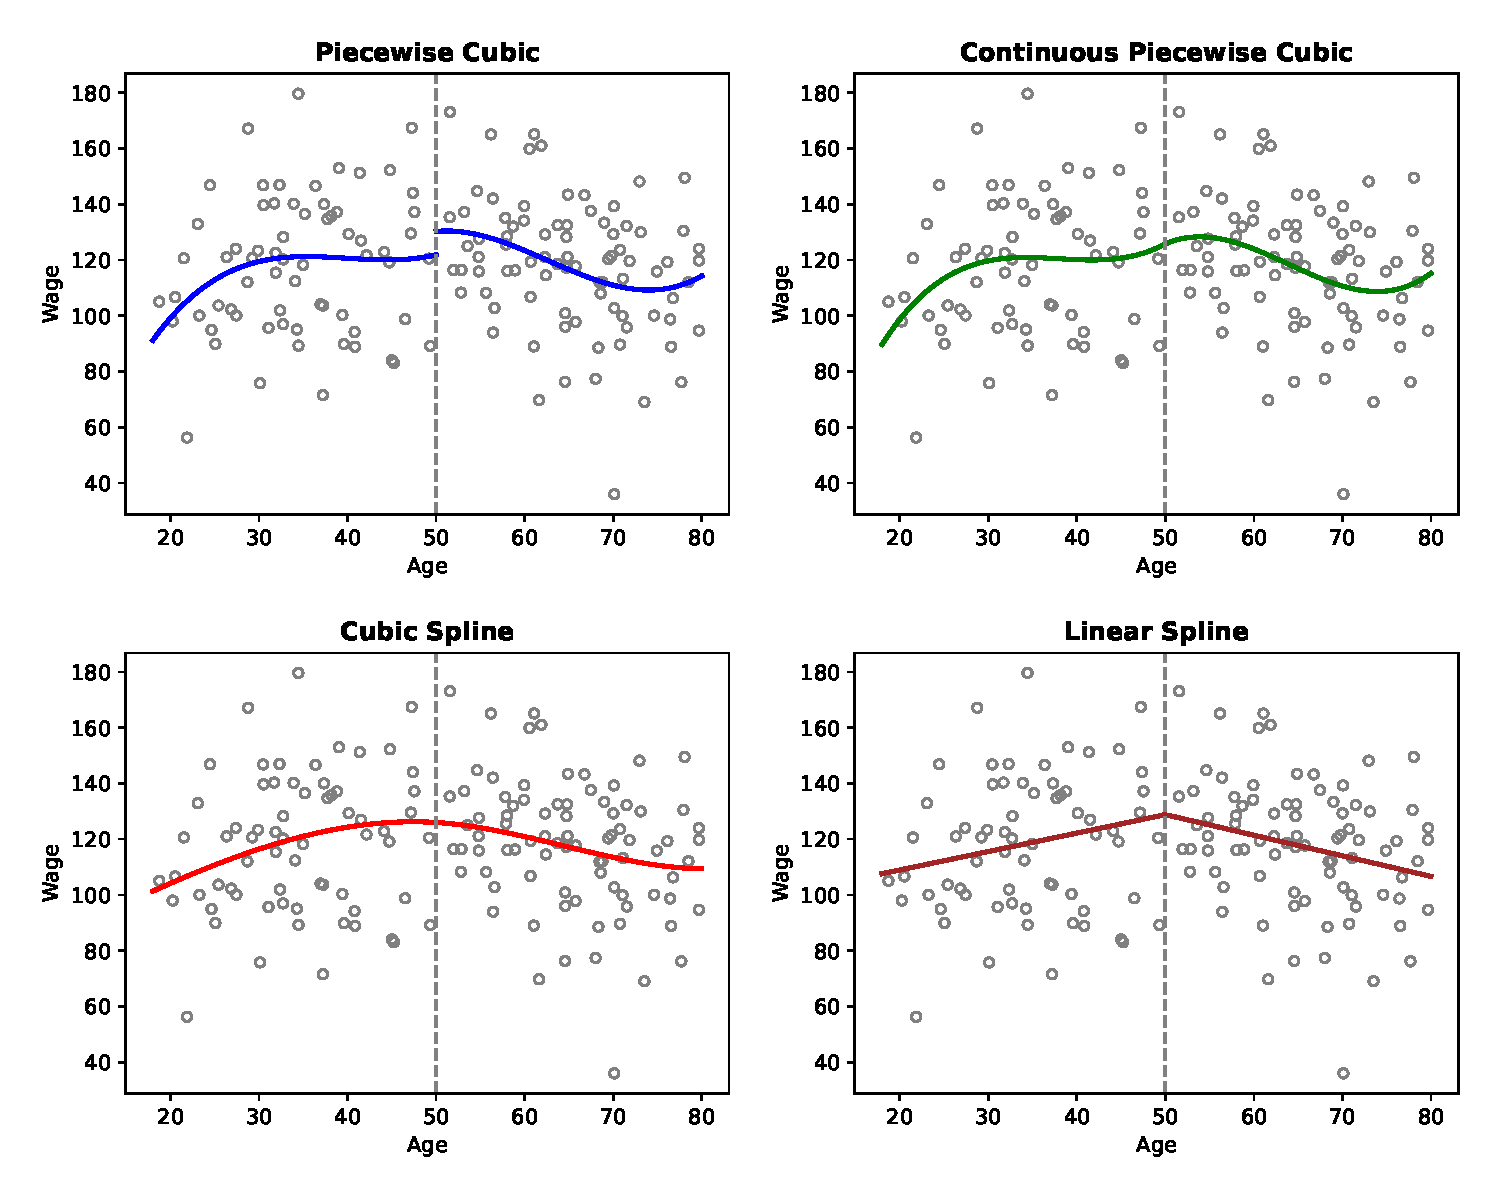
\includegraphics[width=\textwidth]{images/wage_splines_grid.pdf}
    \caption{Comparaison des modèles par splines: constantes par morceaux, continues, cubiques continues, et splines linéaires.}
    \label{fig:wage_splines_grid}
\end{figure}

\subsection{Représentation par Base de Puissances Tronquées}
Pour une spline cubique avec $K$ nœuds, la base est composée de $\{1, x, x^2, x^3\}$ et des fonctions de puissances tronquées:
\begin{equation}
    h(x, \xi) = (x - \xi)_+^3 = \begin{cases} 0 & \text{si } x < \xi \\ (x - \xi)^3 & \text{si } x \ge \xi \end{cases}
\end{equation}
\textbf{($\bigstar$ EXAMEN)} Le nombre total de degrés de liberté (DF) d'une spline cubique est exactement de $K + 4$ (en incluant l'intercept, $3$ pour les parties polynomiales de base, et $K$ pour chaque nœud). Par exemple, pour une spline paramétrée avec $3$ nœuds locaux, il y aura $3 + 4 = 7$ degrés de liberté au total.

\subsection{Splines Naturelles}
Les splines ont tendance à être instables aux bords (forte variance). Les \textbf{splines naturelles} imposent une contrainte de linéarité au-delà des nœuds extrêmes, ce qui stabilise les estimations aux frontières.

\begin{figure}[h]
    \centering
    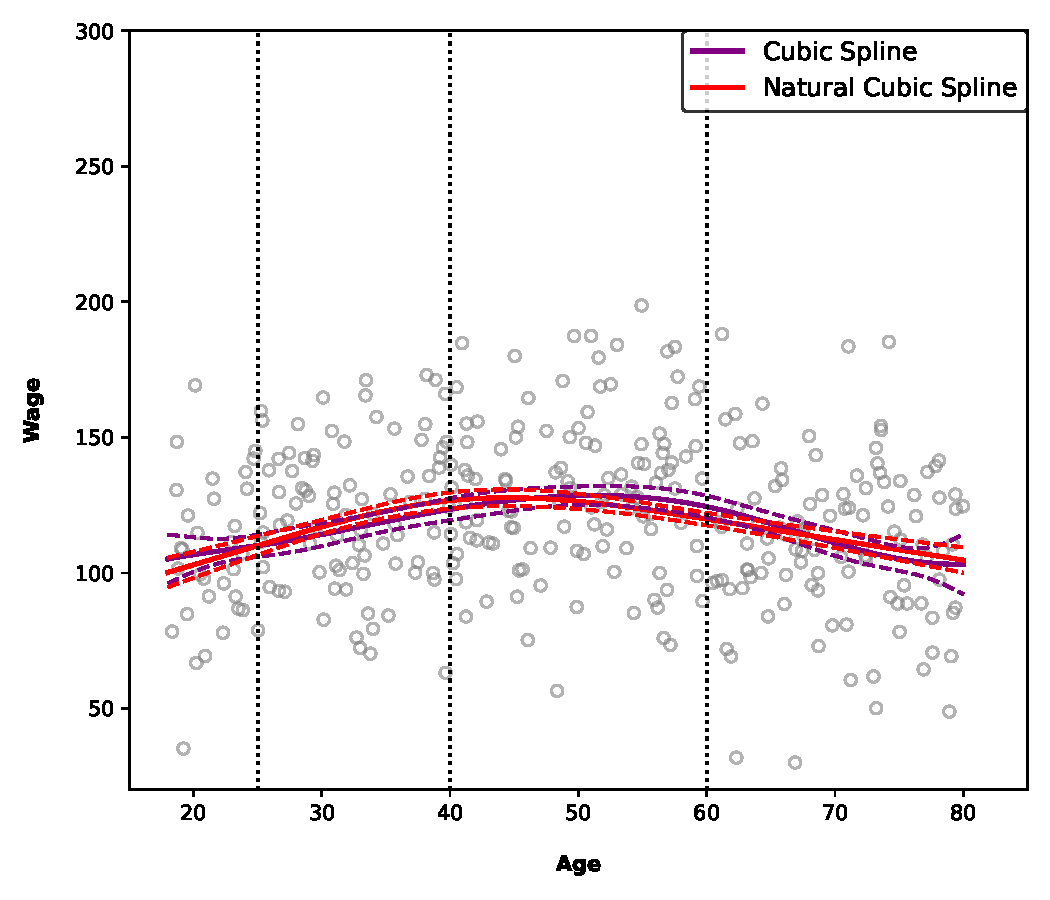
\includegraphics[width=0.7\textwidth]{images/spline_natural_vs_cubic.pdf}
    \caption{Comparaison entre une spline cubique naturelle et une spline cubique standard. Les intervalles de confiance montrent que la spline naturelle est plus stable aux frontières.}
    \label{fig:spline_nat_vs_cub}
\end{figure}

\begin{figure}[h]
    \centering
    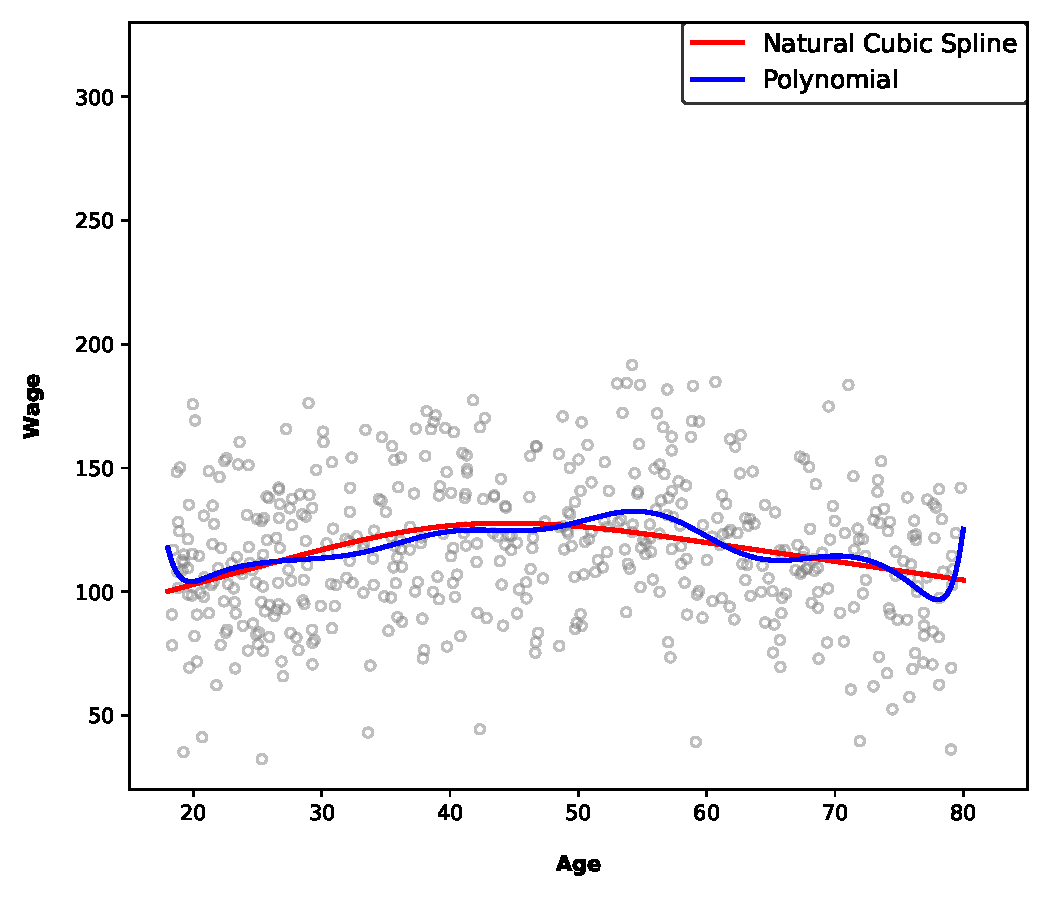
\includegraphics[width=0.7\textwidth]{images/spline_natural_poly.pdf}
    \caption{Instabilité énorme de la régression polynomiale de haut degré aux frontières par rapport à la spline naturelle.}
    \label{fig:spline_nat_poly}
\end{figure}

\textbf{($\bigstar$ EXAMEN) Raisonnement Type - Modèles Non-Linéaires :} Comparé à l'estimateur standard des moindres carrés, un estimateur non-linéaire (comme une spline) est \textbf{plus flexible}. Il \textbf{améliore la précision des prédictions} lorsque la baisse importante de son \textbf{biais} excède l'augmentation de sa \textbf{variance} (\textit{its increase in variance is less than its decrease in bias}).

\begin{figure}[h]
    \centering
    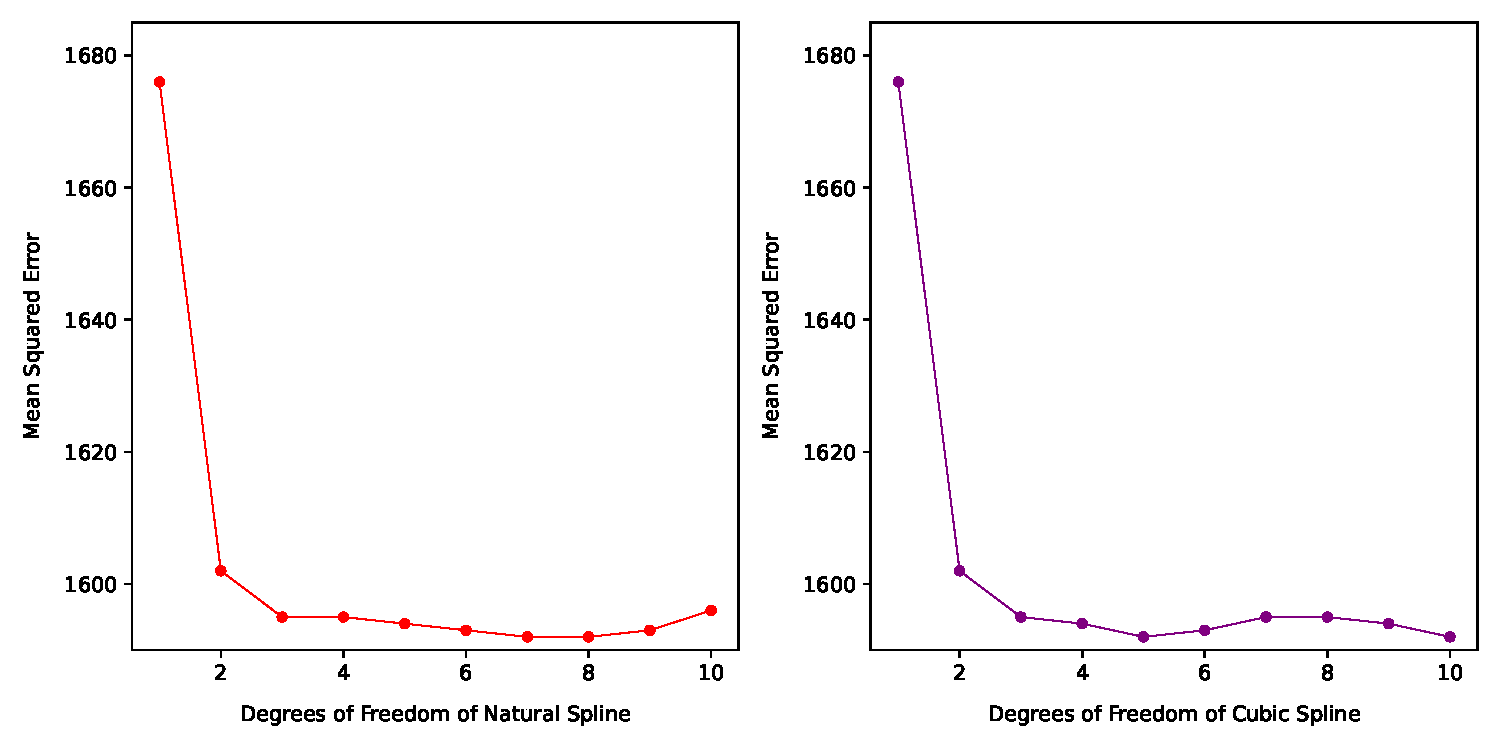
\includegraphics[width=0.9\textwidth]{images/spline_mse_df.pdf}
    \caption{Erreur quadratique moyenne (MSE) en fonction des degrés de liberté pour les splines naturelles et cubiques.}
    \label{fig:spline_mse_df}
\end{figure}

\begin{figure}[h]
    \centering
    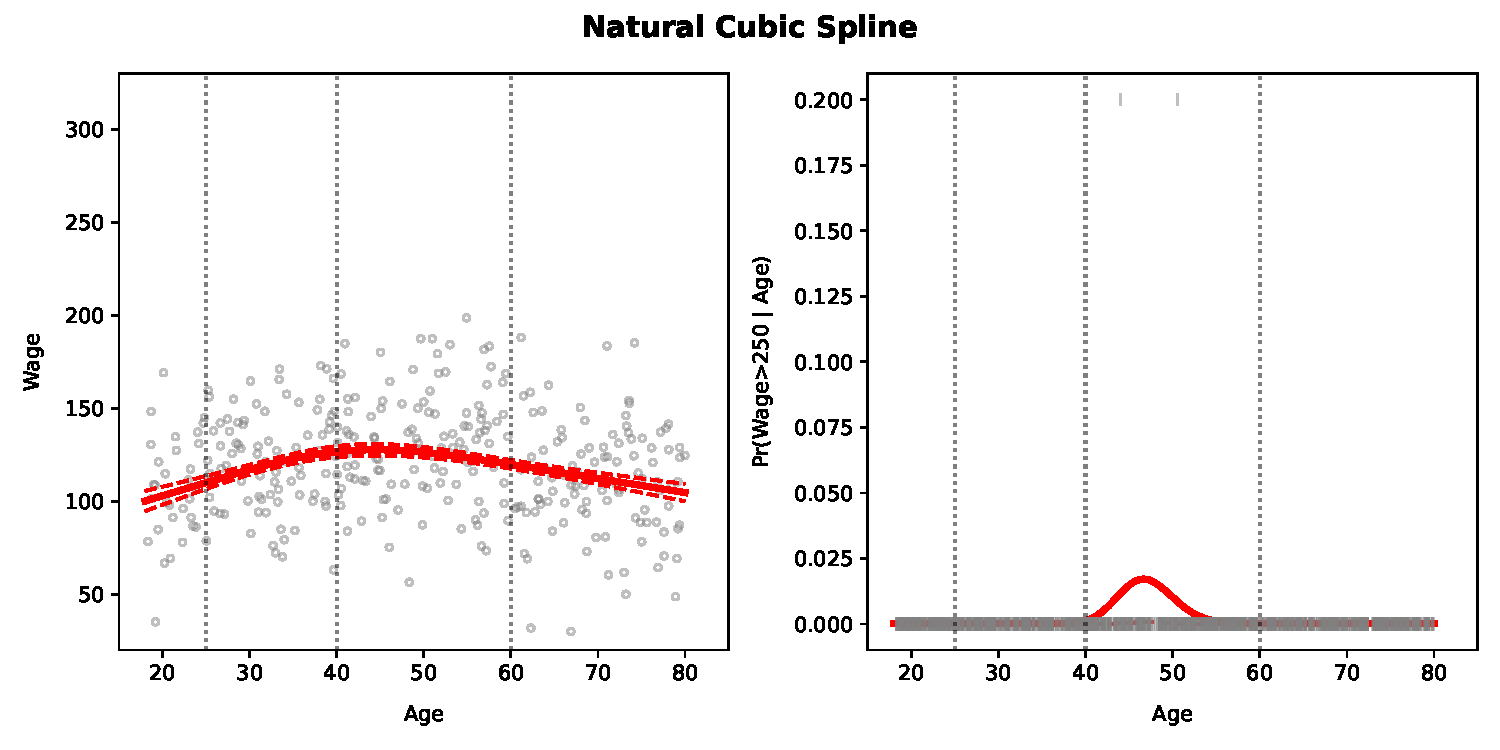
\includegraphics[width=0.9\textwidth]{images/spline_natural_logistic.pdf}
    \caption{Utilisation des splines naturelles pour la régression logistique (classification).}
    \label{fig:spline_nat_logistic}
\end{figure}
\section{Mise en pratique avec R}

\begin{itemize}
    \item \textbf{Régression Polynomiale} : \texttt{lm(y \textasciitilde poly(x, degree))}.
    \item \textbf{Découpage en classes} : \texttt{cut(x, breaks)} pour les fonctions en escalier.
    \item \textbf{B-Splines} : \texttt{library(splines); lm(y \textasciitilde bs(x, knots=...))}.
    \item \textbf{Splines Naturelles} : \texttt{lm(y \textasciitilde ns(x, df=...))}.
\end{itemize}

\textit{Note sur le choix des nœuds} : On peut placer les nœuds uniformément ou aux quantiles des données (ex: 25ème, 50ème, 75ème percentiles) pour avoir plus de flexibilité là où les données sont denses.
